\documentclass[11pt,a4paper]{article}
\usepackage[margin=1in]{geometry}
\usepackage{amsmath,amssymb}
\usepackage{booktabs}
\usepackage{array}
\usepackage{listings}
\usepackage{xcolor}
\definecolor{seclink}{HTML}{1F4E8C}
\usepackage[colorlinks=true,linkcolor=seclink,citecolor=seclink,urlcolor=blue]{hyperref}
\usepackage{parskip}
\usepackage[most]{tcolorbox}
\usepackage{tikz}
\usetikzlibrary{positioning,arrows.meta,fit,backgrounds,calc}

\definecolor{ink}{HTML}{1A1A1A}
\definecolor{grey}{HTML}{5F5B54}
\definecolor{pale}{HTML}{F5F3EE}
\definecolor{yellowbg}{HTML}{FBF3D5}
\definecolor{pinkbg}{HTML}{FADDE1}
\definecolor{tensor}{HTML}{1F6F4A}
\definecolor{seq}{HTML}{1F4E8C}
\definecolor{prod}{HTML}{9C3B1B}
\definecolor{sumc}{HTML}{6B3FA0}
\definecolor{codebg}{RGB}{246,246,244}

\tcbset{plainbg/.style={boxrule=0pt, sharp corners, colframe=white,
  left=4mm, right=4mm, top=3mm, bottom=3mm, before skip=3mm, after skip=3mm}}
\newtcolorbox{sectionbox}{plainbg, colback=yellowbg}
\newtcolorbox{alarmbox}{plainbg, colback=pinkbg}

\tikzset{
  lvl/.style={draw=ink, fill=white, rounded corners=2.5pt, align=center,
              font=\small\ttfamily, inner sep=4.5pt, minimum width=44mm,
              minimum height=8mm},
  leafn/.style={draw=ink, fill=white, rounded corners=2pt, align=center,
                font=\scriptsize\ttfamily, inner sep=3.4pt, minimum height=6mm},
  op/.style={circle, draw, inner sep=0.6pt, minimum size=7mm, font=\small\bfseries},
  ar/.style={-{Stealth[length=1.8mm]}, semithick, color=grey},
  lbl/.style={font=\scriptsize\itshape, color=grey},
}

\lstdefinestyle{code}{
  basicstyle=\ttfamily\small,
  commentstyle=\color{grey}\itshape,
  breaklines=true,
  frame=leftline,
  framesep=7pt,
  xleftmargin=12pt,
  rulecolor=\color{gray!45},
  backgroundcolor=\color{codebg},
  columns=fullflexible,
  showstringspaces=false,
  keepspaces=true,
  literate=
    {↓}{{$\downarrow$}}1 {↑}{{$\uparrow$}}1
    {→}{{$\rightarrow$}}1 {⊠}{{$\boxtimes$}}1
    {◁}{{$\lhd$}}1 {×}{{$\times$}}1 {—}{{\textemdash}}1 {’}{{'}}1,
}
\lstset{style=code}

\newcommand{\seqb}{\lhd^{\ast}}

\title{\vspace{-2em}The Labyrinth}
\author{\normalsize A generated dungeon, decomposed into container combinators}
\date{}

\begin{document}
\maketitle
\vspace{-2em}

\begin{sectionbox}
A party goes down into a labyrinth and comes back up. Monsters guard doors. You must solve
puzzles to open the doors. You must collect puzzle pieces from deep in the dungeon and bring
them back to the monster to solve the puzzle and open the door.

\medskip

You must fight monsters, collect items, sell items and buy weapons. The weapons have different
strengths and properties against different monsters.

\medskip

The levels are generated on the fly. The monsters are language models with a finite set of
actions. You can talk to them. As yet there is no graphics. It is a turn-based game.
\end{sectionbox}

\section{The game}

You have a party, a purse, a sword, a bow and a labyrinth beneath you. The levels have
rooms, the rooms have monsters, and the monsters have to be fought past or talked round. You go
down as far as you dare and then you come back up. When you return to the surface you may sell
the items you have found to buy new weapons.

\subsection{Puzzle pieces}

Scattered through the lower levels are puzzle pieces. Each one is both a \emph{clue} and an
item. It is a thing you pick up and carry, but it cannot be sold, and having it in your hands
tells you something you did not know.

The pieces belong to a puzzle, and the puzzle is somewhere above where they were found. Guarding
it is a monster that does not attack. You give it the pieces you have gathered, and then you try
to solve the puzzle. This is a conversation not a command. You put forward your argument and the
monster decides whether or not to accept it and open the door.

\begin{sectionbox}
That is why the way back matters more than the way down. Nothing you find at the bottom is worth
anything until you have carried it back up, and what you have carried back up is the only thing
that makes new depth reachable. In order to fully explore the labyrinth you must unlock it from
below.
\end{sectionbox}

Three things about it are unusual and all three are the point of building it.

The levels are not written by hand. A specification for a level is generated, and the code for
that level is generated from the specification, and the level is then a program like any other.
So the labyrinth is different every time and nobody has to design it.

The monsters are non-deterministic. Each one is a language model with a finite set of actions,
which you can speak to in plain English. You can threaten them, lie to them,
offer them money or ask them what is down the passage, and what they do about this is their own
business.

The puzzles are non-deterministic too, and nothing in the game knows their answers. A puzzle is
solved when the monster keeping it is persuaded, and being persuaded is the only sense in which
it is solved.

\subsection{The party}

A party is the group of people you take down, and for the purposes of this decomposition it is
one thing rather than several. It has a number of hands, a pool of hit points shared between
them, a stock of experience gained by getting past things, and whatever it is carrying. It acts
once in a round, because the word you type is given to the party and not to a person inside it.
When the note says the party is wounded, it means the pool is low and not that a named
individual is hurt.

That is a decision and not an oversight. A party of three who each act separately would be a
tensor, standing opposite the tensor of monsters facing them, and it would be the better game.
It would also make a round $(a \boxtimes b \boxtimes c) \lhd \text{monsters}$, and every rule
about actions would have to be written per person rather than per party. This note describes the
smaller version, and the larger one is the obvious first thing to add.

\subsection{Multi-party}
\label{sec:multi}

The levels are servers and a server may have many clients, so two parties descending at once is
not a new capability. It is a capability the architecture already has but is not yet using.
Nothing about the two mappings changes: each party is its own descent, its own tree, and its own way back, because
a response goes to whoever asked for it.

What it buys is worth more than it costs. If a party unlocks a door from below, that door is open
when the next party arrives, so the labyrinth is unlocked between them rather than by each of
them separately. Each party can gather separate pieces.

The cost.

A level has to hold state, and once it does, the same prompt no longer gives the same response,
because somebody else has been through. That is the same concession already made for the
monsters rather than a new one. Apparently Neil has a solution for this using \emph{workers}.

If two parties are in the same room at the same time, who goes first? Nothing said so far decides
that. A combinator says how prompts and responses fit together, but it has nothing to say about
whose turn it is.

So a rule has to be chosen, and then an operator will express it. The tidy choice is that the two
parties are a tensor, exactly as the monsters in the room are. Both are prompted with the state
as it stood at the start of the round, both owe a result, and neither of them sees what the other
did until the round is over. Nobody goes first, because they all go at once.

Potentially two parties could reach for the same thing at the same time. This is the ordinary
problem of shared state, but the architecture has solved it already, because each level is one
program with one flow of control. Requests to a level are served one at a time, so the state moves from one
consistent position to the next without anything having to be locked. That is the reason the
whole game is built out of servers rather than function calls in the first place.

\newpage

\section{Containers}

The decomposition that follows is built out of one idea, and this section is all of it. Nothing
here is particular to dungeons.

\subsection{An interface is a pair}

A \emph{container} is an interface, written as two things together. The first is the set of
prompts you may send. The second gives, for each prompt, the type of the response.

The second half is what makes it more than a list. The response's type depends on which prompt was
sent, so a single interface can respond with a number to one question and a list of rooms to
another, and which you get is fixed by what you asked. Write the pair as $(P, R)$, where $P$ is
the prompts and $R\,p$ is the type of response to the prompt $p$.

One condition runs through everything below. The set of prompts must be \emph{finite}. Over a
finite set, a response type that varies with the prompt is just a table, and a table is something an
ordinary type system can write down. Over an infinite set it is not, and none of this works.

\subsection{A morphism is two mappings}

Interfaces are joined by \emph{morphisms}, and a morphism is a pair of mappings going in opposite
directions. Given interfaces $(P, R)$ above and $(Q, T)$ below,

\[ u : P \to Q \qquad\qquad f : (p : P) \to T\,(u\,p) \to R\,p. \]

The mapping $u$ takes a prompt you were given and computes the prompt to send below. The mapping
$f$ takes the response that came back and turns it into the response you owe. Control flows down
through $u$. Data flows back up through $f$.

Read the type of $f$ slowly, because the whole of this note leans on it. It is given the original
prompt \emph{as well as} the response from below, and what it must produce is a response to the original
prompt. So the way back up has access to the way down, and the two are not symmetric.

\subsection{A command-line tool is already a container}

None of this requires a special language. A command-line tool receives one prompt, its argument
vector, and produces a response whose type depends on which prompt it was. Ask one thing and you get
a list of commits. Ask another and you get a working tree. Those are not the same kind of thing,
and which you get is fixed by the word you typed.

That is a container, and it is why the levels in this game are separate programs. One level
reaches the one below it by spawning a command-line tool that carries a prompt to a socket, so
the delegation is a real process with a real boundary rather than a function call wearing a
costume.

\subsection{Nothing checks what crosses}

The boundary is text. A prompt goes out as an argument vector and a response comes back on standard
output, and no type survives the crossing. What arrives is bytes.

So every claim made above is established, if it is established at all, by a \emph{decoder} on the
receiving side: a function which takes what arrived and either produces a value of the type that
was promised or fails. The type says what must be true. The decoder is the only thing that ever
checks it. That is the arrangement throughout this game, and Section~\ref{sec:agents} is where it
matters most, because there the thing on the other side of the boundary is a language model.

\subsection{Down is not the same as up}
\label{sec:updown}

The party that arrives at level four is not the party that entered level three. Gold has been
found, wounds have been taken and lamp oil has been extinguished. That is the mapping $u$.

The mapping $u$ is given one thing and the mapping $f$ is given two. Its type is
$f : (p : P) \to T\,(u\,p) \to R\,p$, so it receives the prompt that went down as well as the
response that came back.

Suppose the party finds a key on level four.
There is a locked door on level three, and the party walked past it on the way in because they
had nothing to open it with. On the way out the mapping $f$ of level three is handed the response
from below, the key is in it, and the door is now a door the party can open.

A puzzle is the same mechanism and it is what the game is built on. A keeper on level two wants
three pieces, and the pieces are on levels four, five and six. The party cannot satisfy it on the
way in and does not need to. The pieces come up through the responses, and the mapping $f$ of level
two is handed them along with everything else, so the argument can be made on the way out and
not before. What the labyrinth is really made of is not the way down. It is what the way down
lets you do on the way back.

\section{The tower}

Eight levels, eight ports, and the same program running on each of them.

\begin{center}
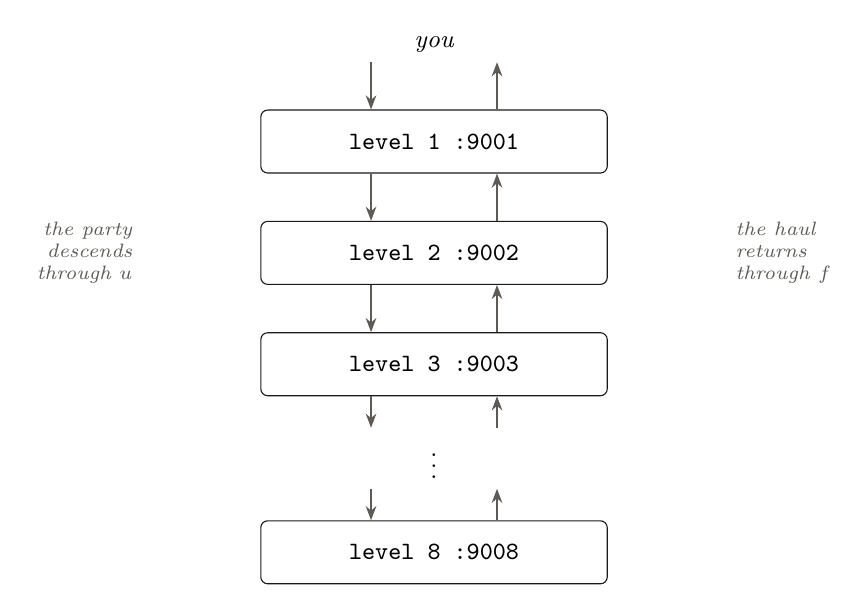
\begin{tikzpicture}[node distance=6mm]
\node[font=\small\itshape] (you) {you};
\node[lvl, below=6mm of you] (l1) {level 1 :9001};
\node[lvl, below=of l1] (l2) {level 2 :9002};
\node[lvl, below=of l2] (l3) {level 3 :9003};
\node[font=\small, below=4mm of l3] (dots) {$\vdots$};
\node[lvl, below=4mm of dots] (l8) {level 8 :9008};

\foreach \a/\b in {you/l1, l1/l2, l2/l3}
  \draw[ar] ($(\a.south)+(-8mm,0)$) -- ($(\b.north)+(-8mm,0)$);
\draw[ar] ($(l3.south)+(-8mm,0)$) -- ($(dots.north)+(-8mm,0)$);
\draw[ar] ($(dots.south)+(-8mm,0)$) -- ($(l8.north)+(-8mm,0)$);

\foreach \a/\b in {l1/you, l2/l1, l3/l2}
  \draw[ar] ($(\a.north)+(8mm,0)$) -- ($(\b.south)+(8mm,0)$);
\draw[ar] ($(dots.north)+(8mm,0)$) -- ($(l3.south)+(8mm,0)$);
\draw[ar] ($(l8.north)+(8mm,0)$) -- ($(dots.south)+(8mm,0)$);

\node[lbl, left=1mm of l2, xshift=-14mm, align=right] {the party\\descends\\through $u$};
\node[lbl, right=1mm of l2, xshift=14mm, align=left] {the haul\\returns\\through $f$};
\end{tikzpicture}
\end{center}

Eight bespoke programs would be a game. The same program composed with itself eight times is a
claim about composition, and the claim is the reason for building it.

The eight are not eight copies of the same content. Each is started with a level specification
and serves whatever that specification describes, so the program is the same and the labyrinth
is not.

\subsection{It could be a tree and not a chain}

The picture above is the simplest case and the equations are already more general than it. Every
level ends in a choice of ways down, and each way leads to a level which ends in a choice of its
own, so what the recursion describes is a tree. Eight in a line is what you get by never
branching.

The depth of that tree is fixed before the game starts, and it is finite. That is not a
concession, it is the condition everything else rests on. A finite depth is what lets a rule
about what may be found at a given depth be a table, and a table is what the type system can
hold. A labyrinth that went down for ever would have no such table, and nothing in
Section~\ref{sec:types} would work.

A tree is a maze with no way of walking in a circle, and that is what this labyrinth is. The
generator may make it as large and as tangled as it likes. What it may not do is join a passage
back onto one the party has already come down, because the way out is the way in reversed and
there is nothing to reverse in a circle.

\section{The decomposition}

Interfaces compose, in four different ways, and all four appear below. A fifth operator appears
too, written $\seqb$. It is the sequential one again, with a second prompt that may be chosen
after the first response arrives, and Section~\ref{sec:agents} explains why that has to be written
by hand rather than taken ready-made.

\begin{center}
\begin{tabular}{@{}c@{\hspace{5mm}}l@{\hspace{5mm}}>{\raggedright\arraybackslash}p{0.52\textwidth}@{}}
\toprule
& \textbf{reads as} & \textbf{what it means here} \\
\midrule
$\boxtimes$   & both, and both respond    & two parts of the game that do not touch each other \\
$\times$      & both offered, one responds & two uses of a thing you have only one of \\
$+$           & one side, chosen first    & the prompt already belongs to one side \\
$\lhd$        & then                      & the second prompt is computed from the first response \\
$\seqb$       & then, with a choice       & the first response decides which side is prompted \\
\bottomrule
\end{tabular}
\end{center}

\subsection{The whole game, as an expression}

\begin{align*}
\text{run}        \;&=\; \text{outfit} \;\lhd\; \text{level}(1) \;\lhd\; \text{market} \\[1.5mm]
\text{outfit}     \;&=\; \text{smith} \;\times\; \text{fletcher} \\[1.5mm]
\text{market}     \;&=\; \text{sell} \;\lhd\; \text{buy} \\[3mm]
\text{level}(d)   \;&=\; \text{rooms}(d) \;\lhd\; \text{way}(d) \\[1.5mm]
\text{rooms}(d)   \;&=\; \text{east}(d) \;\boxtimes\; \text{west}(d) \;\boxtimes\; \text{north}(d) \\[1.5mm]
\text{room}(d)    \;&=\; \text{turn} \;\lhd\; \text{room}(d) \quad\text{until the room is quiet} \\[3mm]
\text{turn}       \;&=\; \text{strike} \;+\; \text{trade} \;+\; \text{move} \;+\; \text{speak} \\[1.5mm]
\text{strike}     \;&=\; \text{action} \;\lhd\; \text{monsters} \\[1.5mm]
\text{action}     \;&=\; \text{sword} \;\times\; \text{bow} \\[1.5mm]
\text{monsters}   \;&=\; m_1 \;\boxtimes\; m_2 \;\boxtimes\; \cdots \;\boxtimes\; m_k \\[3mm]
\text{puzzle}(d)  \;&=\; \text{keeper}(d) \;\seqb\; \bigl( \text{wing}(d) \;+\; \text{refused} \bigr) \\[1.5mm]
\text{way}(d)     \;&=\; \text{mines}(d{+}1) \;+\; \text{caverns}(d{+}1) \\[1.5mm]
\text{way}(8)     \;&=\; \text{the bottom, and nothing below it}
\end{align*}

Every line is one rule of the game, and the next section states which.

\subsection{One rule for each operator}

\begin{center}
\begin{tabular}{@{}l@{\hspace{5mm}}c@{\hspace{5mm}}>{\raggedright\arraybackslash}p{0.48\textwidth}@{}}
\toprule
\textbf{part} & & \textbf{the rule that forces it} \\
\midrule
outfitting        & $\times$   & you only have one purse, so you must choose to either upgrade your sword or upgrade your bow. \\
the market        & $\lhd$     & what you can afford to buy is computed from what you sold. \\
the rooms         & $\boxtimes$ & the stairway will not open until all of the rooms are cleared, and none of the rooms interact with any other. \\
\textbf{a command}& $+$        & \textbf{the options depend on where you are standing, and which of them you type decides who responds.} A blow goes to the monsters, a price goes to the market, a direction goes to the map. The three respond with different kinds of thing. \\
a round           & $\lhd$     & the monsters respond to your attack. Your blow is thrown first and the monsters respond to the result. \\
your weapon       & $\times$   & you can only use one of your weapons at a time, the sword or the bow. \\
the monsters      & $\boxtimes$ & every monster in the room acts at the same time. \\
the way down      & $+$        & the stair goes to the mines and the shaft goes to the flooded caverns. You choose one, and only the one you chose is prompted. \\
\textbf{a puzzle} & $\seqb$    & \textbf{the keeper is asked first, and the keeper's verdict decides what is prompted next.} Persuade it and a wing of the labyrinth is entered. Fail and nothing happens. The verdict is not knowable when the argument is made, which is what makes this the sequential operator and not a choice made in advance. \\
the descent       & $\lhd$     & what waits on level $d{+}1$ is computed from what you did on level $d$. \\
\bottomrule
\end{tabular}
\end{center}

\subsection{The command is the routing}

The player types one word. Where the party is standing decides who is allowed to respond to it, and
the three who might respond do not respond with the same kind of thing.

\begin{center}
\begin{tabular}{@{}l@{\hspace{6mm}}l@{\hspace{6mm}}>{\raggedright\arraybackslash}p{0.40\textwidth}@{}}
\toprule
\textbf{the word} & \textbf{who responds} & \textbf{what comes back} \\
\midrule
\texttt{strike} & the monsters in the room & who was hurt, and by how much \\
\texttt{buy}    & the market on the surface & what you now carry, and what it cost \\
\texttt{north}  & the map of this level     & where the party is now standing \\
\texttt{say}    & whatever is listening      & what it decided to do about that \\
\bottomrule
\end{tabular}
\end{center}

Three interfaces, genuinely different, and the word names which one the prompt belongs to before
it is sent. That is a sum, and unlike the stairway it is a sum on every turn of the game rather
than once a level.

The set of words that exist is itself a function of where you are. In the market there is no
monster to strike, and in a room with a monster in it there is nothing to buy.

\subsection{Fighting}

A round has three parts and each is a different operator.

You act first, and you act with a weapon. The sword is offered and the bow is offered, both at
once, and exactly one of them responds, because there is one pair of hands and it is holding one
of them. That is the product.

Which weapon it is decides more than how hard the blow lands. A bow reaches a monster across the
room and a sword does not, and a sword may parry what is already on top of you.

Then the monsters respond. All of them act, all of them owe a result, and none of them waits for
another to finish, so the monsters in a room are a tensor. A room with two goblins and an ogre is
$m_1 \boxtimes m_2 \boxtimes m_3$, and the independence is enforced rather than promised. All
three prompts have to be built before any is sent, so the ogre's move cannot be computed from
what the first goblin did.

And the round as a whole is sequential. What the monsters do is computed from what you did, which
is the entire reason a round is a round. Guard, and they come on anyway. Strike and miss, and
they come on differently.

\subsection{One level, drawn}

\begin{center}
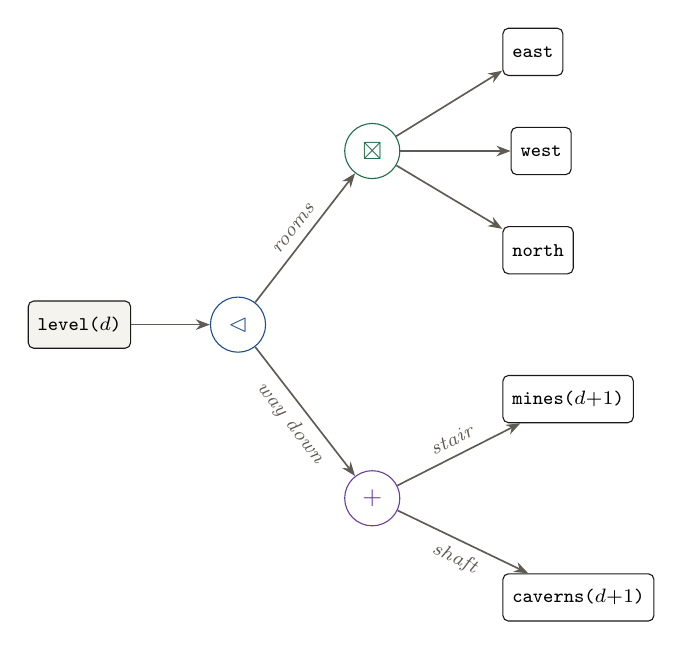
\begin{tikzpicture}[node distance=7mm and 12mm]
\node[leafn, fill=pale] (lev) {level($d$)};
\node[op, draw=seq, text=seq] (s1) [right=10mm of lev] {$\lhd$};
\draw[ar] (lev) -- (s1);

\node[op, draw=tensor, text=tensor] (t1) [above right=17mm and 12mm of s1] {$\boxtimes$};
\node[op, draw=sumc, text=sumc] (p1) [below right=17mm and 12mm of s1] {$+$};
\draw[ar] (s1) -- node[lbl, above, sloped] {rooms} (t1);
\draw[ar] (s1) -- node[lbl, below, sloped] {way down} (p1);

\node[leafn] (east)  [above right=7mm and 14mm of t1] {east};
\node[leafn] (west)  [right=14mm of t1]               {west};
\node[leafn] (north) [below right=7mm and 14mm of t1] {north};
\draw[ar] (t1) -- (east);
\draw[ar] (t1) -- (west);
\draw[ar] (t1) -- (north);

\node[leafn] (stair) [above right=7mm and 14mm of p1] {mines($d{+}1$)};
\node[leafn] (shaft) [below right=7mm and 14mm of p1] {caverns($d{+}1$)};
\draw[ar] (p1) -- node[lbl, above, sloped] {stair} (stair);
\draw[ar] (p1) -- node[lbl, below, sloped] {shaft} (shaft);
\end{tikzpicture}
\end{center}

Read it left to right. The rooms are cleared, and only then is the way down chosen. Each leaf at
the bottom right is another whole level, which is where the recursion is.

\subsection{Where the recursion is}

Only one equation mentions itself.

\[ \text{level}(d) \;=\; \text{rooms}(d) \;\lhd\; \bigl( \text{mines}(d{+}1) + \text{caverns}(d{+}1) \bigr) \]

Expand it eight times and the dungeon is a right-nested chain of sequential compositions with a
tensor hanging off each link. That is the whole architecture in one line, and it is also why the
depth of the delegation and the depth of the dungeon are the same number.

Expanded once it is a chain. Expanded at both ways down it is a tree, and the tree is the
labyrinth. The expansion stops at the depth the game was given, which is why the recursion
terminates and why the tables of Section~\ref{sec:types} exist. What gets built is the path the
party actually took, one level at a time, so a generated child need not exist until somebody
goes that way.

\section{The typed agents}
\label{sec:agents}

The monsters are non-deterministic, and you can talk to them. Two kinds of them matter here: the
ones that fight, and the one that keeps a puzzle.

\subsection{The monsters}

Every monster is a server, and its handler spawns the \texttt{claude} binary and responds with
whatever comes back on standard output. Structurally it is the same thing as every other server
here: a container prompted over a socket, returning a response indexed by the prompt it was
given. The party cannot tell the difference from above, and that is the whole claim. A
command-line tool is already a container, and the Claude Code harness is a command-line tool.

What you send it is what you said, in whatever words you chose. What it sends back is one of a small fixed set of things it can do.

\begin{center}
\begin{tabular}{@{}l@{\hspace{6mm}}>{\raggedright\arraybackslash}p{0.62\textwidth}@{}}
\toprule
\textbf{the prompt} & anything the player types at it \\
\textbf{the response}  & attack, retreat, bargain, answer, or refuse \\
\bottomrule
\end{tabular}
\end{center}

That is a container, and the reason it is a container is the second row. The set of actions is
finite and it is fixed before the conversation starts, so what may come back is a table and a
table is something the type system can write down. A goblin that decides to do a fifth thing has
not surprised the game. It has failed to respond within its own container, and the decoder at the
boundary is where that is caught.

So the whole of the freedom is on the way in and none of it is on the way out. You may say
anything. The goblin may do one of five things about it. A player who talks their way past a
troll has not escaped the type system, they have found the argument that makes a finite set of
actions come out differently.

\begin{sectionbox}
Notice how little is being claimed. Nothing forces a language model to respond with one of five
actions. The type says it must, and the decoder on this side of the boundary is the only thing
that establishes it, exactly as Section~2.4 describes. What the type buys is not a guarantee
about the model. It is that every reader of a monster's response has had to handle five cases and
no more.
\end{sectionbox}

\subsection{The keeper of a puzzle}

One kind of monster does not fight. It sits with a puzzle and it has two things you can do to it.
You can hand it a piece, and you can tell it what you think the pieces mean.

\begin{center}
\begin{tabular}{@{}l@{\hspace{6mm}}>{\raggedright\arraybackslash}p{0.60\textwidth}@{}}
\toprule
\textbf{the prompts} & a piece, or an argument in whatever words you chose \\
\textbf{the responses} & taken, refused, accepted, or a hint \\
\bottomrule
\end{tabular}
\end{center}

The second prompt is the game. Every piece is a clue, so the party arrives holding three or four
things which mean something together, and the player has to say what. Nothing in the program
knows the answer. The keeper reads your answer and decides if it likes it, and if it does, it
opens another wing of the labyrinth. So the composite is

\[ \text{puzzle}(d) \;=\; \text{keeper}(d) \;\seqb\; \bigl( \text{wing}(d) \;+\; \text{refused} \bigr) \]

This is the clearest case of $\seqb$ in the game. The two sides respond with entirely different
things, one being a new part of the labyrinth and the other being a closed way. And which side is
prompted cannot be known when the argument is sent, because it is the keeper who decides. Ask,
then decide. A composite that decided first would be a puzzle whose answer was fixed before it
was attempted.

\subsection{The player is adversarial}

There is an obvious hole and it is worth naming rather than hiding. The keeper is a language
model being argued with by somebody who wants a particular verdict. Players will not confine
themselves to arguing about the clues. They will flatter it, threaten it, claim to be its author
and instruct it to say yes.

Nothing in the type system helps here. The decoder guarantees that whatever comes back is one of
four words, and it has no opinion whatever about whether the fourth was deserved. A keeper that
can be talked into anything is a puzzle with no answer, and that is a problem to be solved in how
the keeper is prompted rather than in how its response is typed.

\subsection{Non-determinism is a good thing}

A server whose responses come from a language model gives up one thing that ordinary servers have. Run it
twice on the same input and it need not say the same thing twice, so a game containing one cannot
be replayed from a seed.

For most programs that is a cost to be managed. Here it is the reason for building it. A
keeper who accepts the same argument every time is not much of a puzzle, and a goblin who
responds to the same threat the same way every time is not worth talking to.

\section{Generating a level}
\label{sec:gen}

A level is a specification and a program written from it. Both can be generated, and the
interesting part is what stops the generated thing from being nonsense.

The compiler stops it. A level has to be a container, which means a finite set of prompts and,
for each prompt, the type of the response. Generated code that does not present one
does not compile, and a level that does not compile is not a level. So the acceptance test for
generated content is not a human reading it. It is \texttt{deno check}.

That is worth stating plainly because it is the part that scales. A generator can write a
labyrinth of any size and most of what it writes will be wrong in the ordinary ways that
generated code is wrong. What it cannot do is produce a level whose monsters respond with
something no monster may respond with, or whose loot is a kind of loot that does not exist at that
depth, because those are the two tables of Section~\ref{sec:types} and the compiler holds them.

\begin{sectionbox}
The finite index earns its keep twice. It is what makes a dependent type expressible in
TypeScript, and it is what makes a generated level checkable. A generator that could invent new
actions and new kinds of loot would be writing a different game every time, and nothing would be
able to tell whether it had.
\end{sectionbox}

Two things about generation this note does not answer. Whether the specification is generated
once and kept, so that a labyrinth can be played twice, or generated on entry so that it never
repeats. And whether the generator is allowed to write the monsters' prompts, which is the
difference between a dungeon that surprises the player and one that surprises its author.

\subsection{When a level is generated}

When is the level generated? A prompt goes down from level $d$ to level $d+1$, and if
nobody has ever been to level $d+1$ then there is nothing there to send it to. Something has to
bring the next level into existence before the delegation can happen at all.

The natural place for that is the mapping $u$, and there is a decent argument that it belongs
there. The mapping $u$ already spawns a process, because that is how a prompt is carried across.
Generating a level is the same act made larger. Write the specification, write the code, check
that it compiles, start it on a port, and only then send the prompt down to it.

\begin{sectionbox}
So descending has a load time, and it is not a rendering delay. The level is being written while
the party stands on the stair.
\end{sectionbox}

\section{The map}

A player will want to see where they have been, and that costs nothing at all.

Every response comes back up through the client that sent the prompt, so a client can keep what
it has been told. Which rooms were on each level, which way down it took, which door it found
locked and could not open. Nothing has to be fetched and nothing has to be asked for twice,
because it has all already gone past on the way home.

None of that has to travel in the prompt. It could be carried in the party record and taken down
with the party, and there would be no reason to, since nothing below needs to know where the
party has been. Leaving it with the client keeps the levels ignorant of who is walking through
them, which is the property that makes Section~\ref{sec:multi} cost so little.

Nor does it contradict anything. No program holds the labyrinth, and a map of where you have been
is not the labyrinth. It is the record of one descent, which is why the trace in
Section~\ref{sec:trace} already is one: the indentation is the depth, and the two columns are the
way down and the way back.

\begin{sectionbox}
And where the levels are generated on entry, the blank part of the map is not concealed. It has
not been written yet. There is nothing there to draw, and nothing anywhere that knows what will
be there, until somebody goes and looks.
\end{sectionbox}

\section{The prompt and the algebra}
\label{sec:carries}

The party is a record, and the record is carried in the prompt. It goes down a level inside the
prompt and it comes back up a level inside the response.

\begin{center}
\begin{tabular}{@{}l@{\hspace{6mm}}>{\raggedright\arraybackslash}p{0.58\textwidth}@{}}
\toprule
\textbf{condition} & healthy, wounded or dying \\
\textbf{gold}      & the purse, which can be spent at the surface \\
\textbf{weapons}   & the sword or the bow, and which is currently being held \\
\textbf{items}     & loot, keys and puzzle pieces \\
\bottomrule
\end{tabular}
\end{center}

Everything else is the algebra. That is the whole point.

\section{Type level enforcement}
\label{sec:types}

The depth of the labyrinth is finite and what items can be found on any given level depends on
the depth. The first two levels hold copper and torches. The middle levels hold silver and
swords. Relics are on the bottom two levels only. Written as a type indexed over depth, this
makes placing a relic on level one impossible for the labyrinth generator to even write down.

The monsters can only perform a finite list of actions, depending on the type of monster, so a
goblin's response is limited to one of the goblin's permitted responses and nothing else. The
player may say anything at all. And the goblin may reply, but it can only perform a fixed set of
actions.

A third table is indexed by where the party is standing. In the market there is no monster to
strike and in a room with a monster in it there is nothing to buy, so which words exist is a
function of the location.

A fourth table is indexed by what weapon is being wielded, because a bow shoots across a room
while a sword is short ranged.

A fifth table is indexed by what the party is carrying. A puzzle can only be solved if you hold
the right pieces. A party holding only two out of three pieces cannot convince the puzzle monster
to open the door with any argument.

The point in all five cases is that an illegal move is not something the game refuses when you
try it. It is something you cannot even write down.

\section{What the trace should look like}
\label{sec:trace}

The trace is one line per hop, written to standard error, indented by depth. In this game the
indentation is the dungeon.

\begin{lstlisting}[breaklines=false, basicstyle=\ttfamily\footnotesize]
 ↓ level1     Descend party={hp:12, wielding:"sword", held:[]}
  ↓ level1     (east (x) west) (x) north
  ↓ level1     (strike + trade + move + speak)
    ↓ combat     (sword x bow) <| (goblin (x) goblin (x) ogre)
    ↑ combat     {hit:["goblin"], taken:1}
  ↓ level2     Descend party={hp:11, wielding:"sword", held:[]}
    ↓ level2     (mines + caverns)
    ↓ level3     Descend party={hp:9, wielding:"bow", held:[]}
      ↑ level3     {hp:7, held:["brass key"]}
    ↑ level2     {hp:7, held:["brass key","silver"], opened:"the locked door"}
  ↑ level1     {hp:6, held:["brass key","silver"]}
\end{lstlisting}

Read the two columns. Everything descending is a party getting worse. Everything ascending is a
haul getting larger, because each level on the way out adds whatever the key coming up has just
let it open. The silver on the second line up was behind the door, and the door was opened by
something found beneath it.

\section{The smallest thing worth building}

Three levels, one room each, written by hand, with no generator and no talking monsters.
Descend, take one piece of loot, come back. Make what the way out does visible in the trace, and
make the whole of it fit on one screen.

Then one locked door and one key below it, because that is the whole argument of
Section~\ref{sec:updown} in a form a player can feel. Then one puzzle: three pieces below, one
keeper above, and one wing that opens if it is persuaded. That is the game's loop, and everything
else is content hung on it.

The order after that would be the command as a sum, because it is the operator with the most
work to do and the one a player meets on every turn. Then a round of fighting, which is the
product and the tensor and the chain in one place. Then one monster you can talk to, which is
the first part needing anything outside the standard library. Then the generator, last of all,
because everything before it is what the generator has to produce.

\end{document}
